\section{Engine\-Interface Class Reference}
\label{classEngineInterface}\index{EngineInterface@{EngineInterface}}
Abstract class for all engines.  


{\tt \#include $<$engineinterface.hpp$>$}

Inheritance diagram for Engine\-Interface::\begin{figure}[H]
\begin{center}
\leavevmode
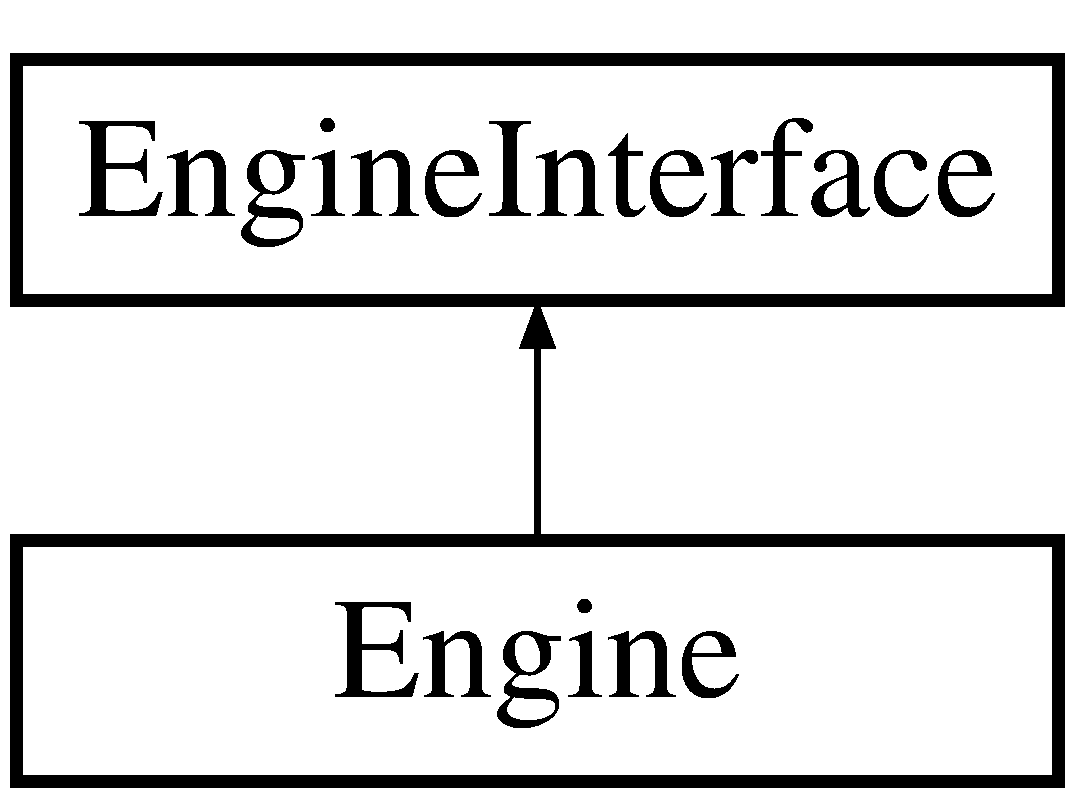
\includegraphics[height=2cm]{classEngineInterface}
\end{center}
\end{figure}
\subsection*{Public Member Functions}
\begin{CompactItemize}
\item 
virtual void {\bf change\-Map} ({\bf Game\-Map} $\ast$map)=0
\item 
virtual void {\bf monster\-Moved} ({\bf Monster} \&monster, int dx, int dy)=0
\item 
virtual void {\bf monster\-Moved\-To} ({\bf Monster} \&monster, int old\-X, int old\-Y)=0
\item 
virtual void {\bf repaint\-Stats} ({\bf Monster} \&monster)=0
\item 
virtual void {\bf update\-Square} (int x, int y)=0
\item 
virtual QBit\-Array {\bf get\-Pickup\-Selection} (const {\bf Items\-List} items)=0
\item 
virtual void {\bf manage\-Equipment} ({\bf Monster} $\ast$monster)=0
\item 
virtual bool {\bf ask\-Player\-Yes\-No} (const QString \&caption, const QString \&text)=0
\item 
virtual void {\bf focus} (int x, int y)=0
\end{CompactItemize}


\subsection{Detailed Description}
Abstract class for all engines. 



\subsection{Member Function Documentation}
\index{EngineInterface@{Engine\-Interface}!askPlayerYesNo@{askPlayerYesNo}}
\index{askPlayerYesNo@{askPlayerYesNo}!EngineInterface@{Engine\-Interface}}
\subsubsection{\setlength{\rightskip}{0pt plus 5cm}virtual bool ask\-Player\-Yes\-No (const QString \& {\em caption}, const QString \& {\em text})\hspace{0.3cm}{\tt  [pure virtual]}}\label{classEngineInterface_a7}




Implemented in {\bf Engine} {\rm (p.\,\pageref{classEngine_a11})}.\index{EngineInterface@{Engine\-Interface}!changeMap@{changeMap}}
\index{changeMap@{changeMap}!EngineInterface@{Engine\-Interface}}
\subsubsection{\setlength{\rightskip}{0pt plus 5cm}virtual void change\-Map ({\bf Game\-Map} $\ast$ {\em map})\hspace{0.3cm}{\tt  [pure virtual]}}\label{classEngineInterface_a0}




Implemented in {\bf Engine} {\rm (p.\,\pageref{classEngine_a2})}.\index{EngineInterface@{Engine\-Interface}!focus@{focus}}
\index{focus@{focus}!EngineInterface@{Engine\-Interface}}
\subsubsection{\setlength{\rightskip}{0pt plus 5cm}virtual void focus (int {\em x}, int {\em y})\hspace{0.3cm}{\tt  [pure virtual]}}\label{classEngineInterface_a8}




Implemented in {\bf Engine} {\rm (p.\,\pageref{classEngine_i0})}.\index{EngineInterface@{Engine\-Interface}!getPickupSelection@{getPickupSelection}}
\index{getPickupSelection@{getPickupSelection}!EngineInterface@{Engine\-Interface}}
\subsubsection{\setlength{\rightskip}{0pt plus 5cm}virtual QBit\-Array get\-Pickup\-Selection (const {\bf Items\-List} {\em items})\hspace{0.3cm}{\tt  [pure virtual]}}\label{classEngineInterface_a5}




Implemented in {\bf Engine} {\rm (p.\,\pageref{classEngine_a7})}.\index{EngineInterface@{Engine\-Interface}!manageEquipment@{manageEquipment}}
\index{manageEquipment@{manageEquipment}!EngineInterface@{Engine\-Interface}}
\subsubsection{\setlength{\rightskip}{0pt plus 5cm}virtual void manage\-Equipment ({\bf Monster} $\ast$ {\em monster})\hspace{0.3cm}{\tt  [pure virtual]}}\label{classEngineInterface_a6}




Implemented in {\bf Engine} {\rm (p.\,\pageref{classEngine_a8})}.\index{EngineInterface@{Engine\-Interface}!monsterMoved@{monsterMoved}}
\index{monsterMoved@{monsterMoved}!EngineInterface@{Engine\-Interface}}
\subsubsection{\setlength{\rightskip}{0pt plus 5cm}virtual void monster\-Moved ({\bf Monster} \& {\em monster}, int {\em dx}, int {\em dy})\hspace{0.3cm}{\tt  [pure virtual]}}\label{classEngineInterface_a1}




Implemented in {\bf Engine} {\rm (p.\,\pageref{classEngine_a3})}.\index{EngineInterface@{Engine\-Interface}!monsterMovedTo@{monsterMovedTo}}
\index{monsterMovedTo@{monsterMovedTo}!EngineInterface@{Engine\-Interface}}
\subsubsection{\setlength{\rightskip}{0pt plus 5cm}virtual void monster\-Moved\-To ({\bf Monster} \& {\em monster}, int {\em old\-X}, int {\em old\-Y})\hspace{0.3cm}{\tt  [pure virtual]}}\label{classEngineInterface_a2}




Implemented in {\bf Engine} {\rm (p.\,\pageref{classEngine_a4})}.\index{EngineInterface@{Engine\-Interface}!repaintStats@{repaintStats}}
\index{repaintStats@{repaintStats}!EngineInterface@{Engine\-Interface}}
\subsubsection{\setlength{\rightskip}{0pt plus 5cm}virtual void repaint\-Stats ({\bf Monster} \& {\em monster})\hspace{0.3cm}{\tt  [pure virtual]}}\label{classEngineInterface_a3}




Implemented in {\bf Engine} {\rm (p.\,\pageref{classEngine_a5})}.\index{EngineInterface@{Engine\-Interface}!updateSquare@{updateSquare}}
\index{updateSquare@{updateSquare}!EngineInterface@{Engine\-Interface}}
\subsubsection{\setlength{\rightskip}{0pt plus 5cm}virtual void update\-Square (int {\em x}, int {\em y})\hspace{0.3cm}{\tt  [pure virtual]}}\label{classEngineInterface_a4}




Implemented in {\bf Engine} {\rm (p.\,\pageref{classEngine_a6})}.

The documentation for this class was generated from the following file:\begin{CompactItemize}
\item 
{\bf engineinterface.hpp}\end{CompactItemize}
